% Options for packages loaded elsewhere
\PassOptionsToPackage{unicode}{hyperref}
\PassOptionsToPackage{hyphens}{url}
%
\documentclass[
]{article}
\usepackage{amsmath,amssymb}
\usepackage{lmodern}
\usepackage{ifxetex,ifluatex}
\ifnum 0\ifxetex 1\fi\ifluatex 1\fi=0 % if pdftex
  \usepackage[T1]{fontenc}
  \usepackage[utf8]{inputenc}
  \usepackage{textcomp} % provide euro and other symbols
\else % if luatex or xetex
  \usepackage{unicode-math}
  \defaultfontfeatures{Scale=MatchLowercase}
  \defaultfontfeatures[\rmfamily]{Ligatures=TeX,Scale=1}
\fi
% Use upquote if available, for straight quotes in verbatim environments
\IfFileExists{upquote.sty}{\usepackage{upquote}}{}
\IfFileExists{microtype.sty}{% use microtype if available
  \usepackage[]{microtype}
  \UseMicrotypeSet[protrusion]{basicmath} % disable protrusion for tt fonts
}{}
\makeatletter
\@ifundefined{KOMAClassName}{% if non-KOMA class
  \IfFileExists{parskip.sty}{%
    \usepackage{parskip}
  }{% else
    \setlength{\parindent}{0pt}
    \setlength{\parskip}{6pt plus 2pt minus 1pt}}
}{% if KOMA class
  \KOMAoptions{parskip=half}}
\makeatother
\usepackage{xcolor}
\IfFileExists{xurl.sty}{\usepackage{xurl}}{} % add URL line breaks if available
\IfFileExists{bookmark.sty}{\usepackage{bookmark}}{\usepackage{hyperref}}
\hypersetup{
  pdftitle={Statistics Assignment},
  hidelinks,
  pdfcreator={LaTeX via pandoc}}
\urlstyle{same} % disable monospaced font for URLs
\usepackage[margin=1in]{geometry}
\usepackage{color}
\usepackage{fancyvrb}
\newcommand{\VerbBar}{|}
\newcommand{\VERB}{\Verb[commandchars=\\\{\}]}
\DefineVerbatimEnvironment{Highlighting}{Verbatim}{commandchars=\\\{\}}
% Add ',fontsize=\small' for more characters per line
\usepackage{framed}
\definecolor{shadecolor}{RGB}{248,248,248}
\newenvironment{Shaded}{\begin{snugshade}}{\end{snugshade}}
\newcommand{\AlertTok}[1]{\textcolor[rgb]{0.94,0.16,0.16}{#1}}
\newcommand{\AnnotationTok}[1]{\textcolor[rgb]{0.56,0.35,0.01}{\textbf{\textit{#1}}}}
\newcommand{\AttributeTok}[1]{\textcolor[rgb]{0.77,0.63,0.00}{#1}}
\newcommand{\BaseNTok}[1]{\textcolor[rgb]{0.00,0.00,0.81}{#1}}
\newcommand{\BuiltInTok}[1]{#1}
\newcommand{\CharTok}[1]{\textcolor[rgb]{0.31,0.60,0.02}{#1}}
\newcommand{\CommentTok}[1]{\textcolor[rgb]{0.56,0.35,0.01}{\textit{#1}}}
\newcommand{\CommentVarTok}[1]{\textcolor[rgb]{0.56,0.35,0.01}{\textbf{\textit{#1}}}}
\newcommand{\ConstantTok}[1]{\textcolor[rgb]{0.00,0.00,0.00}{#1}}
\newcommand{\ControlFlowTok}[1]{\textcolor[rgb]{0.13,0.29,0.53}{\textbf{#1}}}
\newcommand{\DataTypeTok}[1]{\textcolor[rgb]{0.13,0.29,0.53}{#1}}
\newcommand{\DecValTok}[1]{\textcolor[rgb]{0.00,0.00,0.81}{#1}}
\newcommand{\DocumentationTok}[1]{\textcolor[rgb]{0.56,0.35,0.01}{\textbf{\textit{#1}}}}
\newcommand{\ErrorTok}[1]{\textcolor[rgb]{0.64,0.00,0.00}{\textbf{#1}}}
\newcommand{\ExtensionTok}[1]{#1}
\newcommand{\FloatTok}[1]{\textcolor[rgb]{0.00,0.00,0.81}{#1}}
\newcommand{\FunctionTok}[1]{\textcolor[rgb]{0.00,0.00,0.00}{#1}}
\newcommand{\ImportTok}[1]{#1}
\newcommand{\InformationTok}[1]{\textcolor[rgb]{0.56,0.35,0.01}{\textbf{\textit{#1}}}}
\newcommand{\KeywordTok}[1]{\textcolor[rgb]{0.13,0.29,0.53}{\textbf{#1}}}
\newcommand{\NormalTok}[1]{#1}
\newcommand{\OperatorTok}[1]{\textcolor[rgb]{0.81,0.36,0.00}{\textbf{#1}}}
\newcommand{\OtherTok}[1]{\textcolor[rgb]{0.56,0.35,0.01}{#1}}
\newcommand{\PreprocessorTok}[1]{\textcolor[rgb]{0.56,0.35,0.01}{\textit{#1}}}
\newcommand{\RegionMarkerTok}[1]{#1}
\newcommand{\SpecialCharTok}[1]{\textcolor[rgb]{0.00,0.00,0.00}{#1}}
\newcommand{\SpecialStringTok}[1]{\textcolor[rgb]{0.31,0.60,0.02}{#1}}
\newcommand{\StringTok}[1]{\textcolor[rgb]{0.31,0.60,0.02}{#1}}
\newcommand{\VariableTok}[1]{\textcolor[rgb]{0.00,0.00,0.00}{#1}}
\newcommand{\VerbatimStringTok}[1]{\textcolor[rgb]{0.31,0.60,0.02}{#1}}
\newcommand{\WarningTok}[1]{\textcolor[rgb]{0.56,0.35,0.01}{\textbf{\textit{#1}}}}
\usepackage{graphicx}
\makeatletter
\def\maxwidth{\ifdim\Gin@nat@width>\linewidth\linewidth\else\Gin@nat@width\fi}
\def\maxheight{\ifdim\Gin@nat@height>\textheight\textheight\else\Gin@nat@height\fi}
\makeatother
% Scale images if necessary, so that they will not overflow the page
% margins by default, and it is still possible to overwrite the defaults
% using explicit options in \includegraphics[width, height, ...]{}
\setkeys{Gin}{width=\maxwidth,height=\maxheight,keepaspectratio}
% Set default figure placement to htbp
\makeatletter
\def\fps@figure{htbp}
\makeatother
\setlength{\emergencystretch}{3em} % prevent overfull lines
\providecommand{\tightlist}{%
  \setlength{\itemsep}{0pt}\setlength{\parskip}{0pt}}
\setcounter{secnumdepth}{-\maxdimen} % remove section numbering
\ifluatex
  \usepackage{selnolig}  % disable illegal ligatures
\fi
\newlength{\cslhangindent}
\setlength{\cslhangindent}{1.5em}
\newlength{\csllabelwidth}
\setlength{\csllabelwidth}{3em}
\newenvironment{CSLReferences}[2] % #1 hanging-ident, #2 entry spacing
 {% don't indent paragraphs
  \setlength{\parindent}{0pt}
  % turn on hanging indent if param 1 is 1
  \ifodd #1 \everypar{\setlength{\hangindent}{\cslhangindent}}\ignorespaces\fi
  % set entry spacing
  \ifnum #2 > 0
  \setlength{\parskip}{#2\baselineskip}
  \fi
 }%
 {}
\usepackage{calc}
\newcommand{\CSLBlock}[1]{#1\hfill\break}
\newcommand{\CSLLeftMargin}[1]{\parbox[t]{\csllabelwidth}{#1}}
\newcommand{\CSLRightInline}[1]{\parbox[t]{\linewidth - \csllabelwidth}{#1}\break}
\newcommand{\CSLIndent}[1]{\hspace{\cslhangindent}#1}

\title{Statistics Assignment}
\author{Giampietro Ciancio 965991\\
Riccardo Valenti 979784}
\date{}

\begin{document}
\maketitle

\hypertarget{stock-description-data-collection-and-notation}{%
\subsubsection{Stock description, data collection and
notation}\label{stock-description-data-collection-and-notation}}

We start collectin data from the \texttt{tidyquant} stocks database.
We'll be using Pinterest stock closing price from the IPO date (April
18, 2019) until the end of 2021 (December 31, 2021). Pinterest is an
image sharing and social media service designed to enable saving and
discovery of information on the internet using image. The statistical
unit is the day, the variable is the price and the unit of measure of
the price is dollar. We define the IPO date as \(t=1\) and the last day
of 2021 as \(T\). Hence, the stock closing price at \(t=1\) will be
denoted as \(P_1\), the last closing price as \(P_T\) and the generic
day closing price as \(P_t\). We download the data and pipe it to
extrapolate only the \texttt{close} column which we assign to vector
\texttt{price}.

\begin{Shaded}
\begin{Highlighting}[]
\NormalTok{price }\OtherTok{\textless{}{-}} \FunctionTok{tq\_get}\NormalTok{(}\StringTok{"PINS"}\NormalTok{, }\AttributeTok{get =} \StringTok{"stock.prices"}\NormalTok{, }\AttributeTok{from =} \StringTok{"2019{-}04{-}18"}\NormalTok{, }\AttributeTok{to =} \StringTok{"2021{-}12{-}31"}\NormalTok{) }\SpecialCharTok{\%\textgreater{}\%} 
\NormalTok{  .}\SpecialCharTok{$}\NormalTok{close}
\FunctionTok{head}\NormalTok{(price)}
\end{Highlighting}
\end{Shaded}

\begin{verbatim}
## [1] 24.40 24.99 25.85 26.80 28.80 29.85
\end{verbatim}

\hypertarget{daily-closing-price}{%
\subsubsection{Daily Closing Price}\label{daily-closing-price}}

We plot the data as a line having \(t\) on the x axis and \(P_t\) on y
axis.

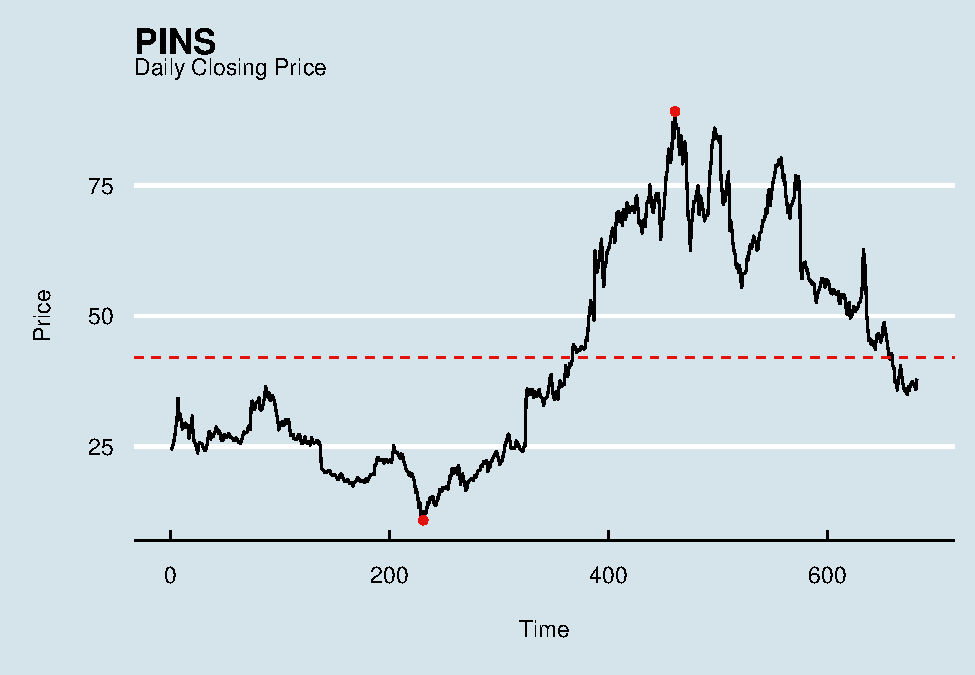
\includegraphics[width=0.8\linewidth]{StatsAssignment_files/figure-latex/plot-1}

From the plot we observe the evolution of the stock price within the
above said interval. After the IPO, the stock prices moved in the
interval between 25\$ and 35\$, before plunging from the 100th day
circa. After day 200, the stock price showed a sign of recovery and then
fell again reaching its minimum shortly after. From that point on, the
stock prices showed a sharp and constant growth until the 400th day,
from which it slowed down for a while and then start growing even faster
reaching the maximum price at day 450 circa. The stock then showed a
very high volatility, creating both positive and negative spike in an
overall decreasing trend. The average closing price of the stock is 40\$
circa and we can approximately say that the stock price have been lower
than mean in the first half of the period and greater in the second
half.

\hypertarget{daily-log-return}{%
\subsubsection{Daily Log Return}\label{daily-log-return}}

We plot the data as a line having \(t\) on the x axis and \(r_t\) on y
axis.

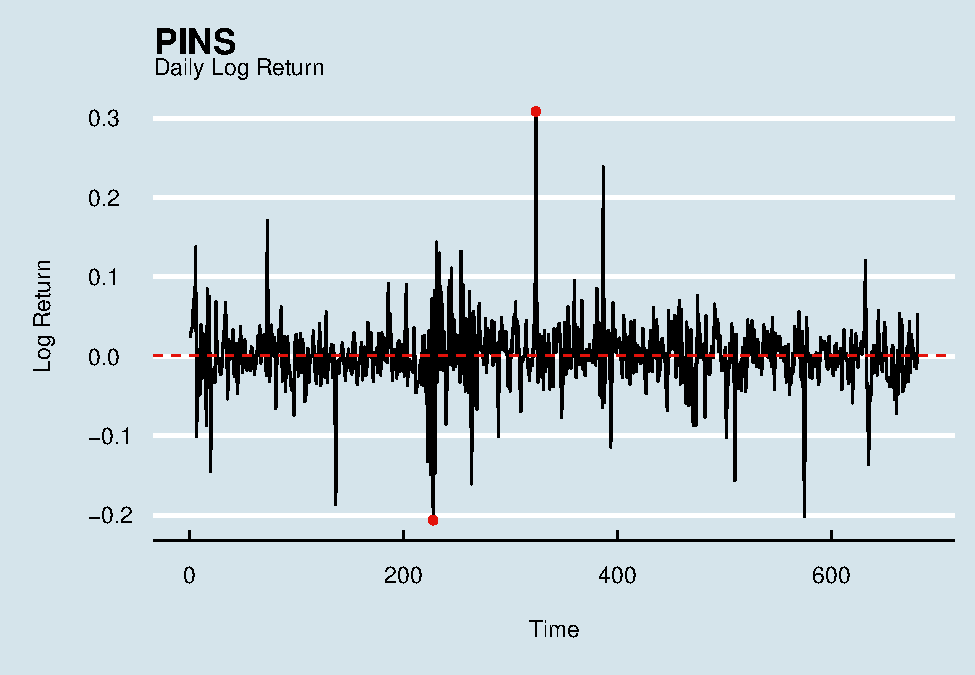
\includegraphics[width=0.8\linewidth]{StatsAssignment_files/figure-latex/log return-1}

From the plot we can observe the Daily Log Return of the stock. Most of
\(r_t\) belong to the interval \([-0.1, 0.1]\). However, spikes can
reach up to -0.2 and 0.3. We observe that the worst day (in terms of
return) is at day 200 circa, around the same time in which the stock
price reached its minimum. The stock showed the best return on the 320th
day circa, hence contributing in the strong price growth from day 200 to
day 400 circa. The Log Return visualization offer a plot similar to the
one we can obtain using simple return
(\(\frac{P_t - P_{t-1}}{P_{t-1}}\)). However, Log Return and Simple
Return show similar value only if the ratio of prices
(\(\frac{P_t}{P_{t-1}}\)) belongs approximately to the interval
\([0.95, 1.10]\) (Appendix A). Given a ratio not belonging in the said
interval, Log Return will produce a lower value than simple return if
the ratio is positive and greater value (in absolute term) if the ratio
is negative. The Log Return visualization do not interfere with the sign
of the simple return. Whenever \(\frac{P_t}{P_{t-1}} < 1\) both simple
and log return will show a negative value; vice versa for
\(\frac{P_t}{P_{t-1}} > 1\).

\hypertarget{mean}{%
\subsubsection{Mean}\label{mean}}

\begin{Shaded}
\begin{Highlighting}[]
\NormalTok{m}\FloatTok{.1}
\end{Highlighting}
\end{Shaded}

\begin{verbatim}
## [1] 0.0005699206
\end{verbatim}

\begin{Shaded}
\begin{Highlighting}[]
\NormalTok{m}\FloatTok{.2}
\end{Highlighting}
\end{Shaded}

\begin{verbatim}
## [1] 0.0006144026
\end{verbatim}

Both means show small positive values. We can use
\textit{Time Additivity} feature and the mean of Log Return to gain
interesting insight on the overall return of the stock.
\textit{Time Additivity} tells us that it is possible to compute the
overall Log Returns from \(t\) to \(t+k\) just by adding the daily Log
Return from \(t\) to \(t+k\). The \texttt{m.1} gives us
\(\frac{\sum_{t=1}^{n_r-1} r_t}{n_r-1}\). Thus, we can compute the Log
Return from \(t=1\) to \(T-1\) as follow:

\begin{Shaded}
\begin{Highlighting}[]
\NormalTok{m}\FloatTok{.1}\SpecialCharTok{*}\FunctionTok{NROW}\NormalTok{(log.rt}\FloatTok{.1}\NormalTok{)}
\end{Highlighting}
\end{Shaded}

\begin{verbatim}
## [1] 0.387546
\end{verbatim}

Given what we said previously, this Log Return is not a good
approximation of the Simple Return. Using the formula \(R=e^{r}-1\) we
can recover the Simple Return of Pinterest Stock from the IPO date until
the end of 2021.

\begin{Shaded}
\begin{Highlighting}[]
\FunctionTok{exp}\NormalTok{(m}\FloatTok{.1}\SpecialCharTok{*}\FunctionTok{NROW}\NormalTok{(log.rt}\FloatTok{.1}\NormalTok{))}\SpecialCharTok{{-}}\DecValTok{1}
\end{Highlighting}
\end{Shaded}

\begin{verbatim}
## [1] 0.4733607
\end{verbatim}

The same reasoning can be applied to \texttt{m.2} in order to recover
the Log Return and Simple Return from \(t=2\) to \(T\).

\hypertarget{standard-deviation}{%
\subsubsection{Standard deviation}\label{standard-deviation}}

\begin{Shaded}
\begin{Highlighting}[]
\NormalTok{s}\FloatTok{.1}
\end{Highlighting}
\end{Shaded}

\begin{verbatim}
## [1] 0.04283665
\end{verbatim}

\begin{Shaded}
\begin{Highlighting}[]
\NormalTok{s}\FloatTok{.2}
\end{Highlighting}
\end{Shaded}

\begin{verbatim}
## [1] 0.04287659
\end{verbatim}

Both Standard Deviations present small similar values. This means that
the most of the Log Return are concentrated around the mean. However, we
need to take in consideration the nature of the data in order to draw
useful insight from standard deviation. We showed previously that the
most of Log Return belong to the interval \([-0.1, 0.1]\) and both
\texttt{m.1} and \texttt{m.2} are very small values. Given this
information, we can say that Standard Deviation (0.05 circa) is quite
high relatively to the Mean. We may refer to the Standard Deviation of
daily return as Historical Daily Volatility. We can conclude that
Pinterest stock presents a relatively high daily volatility.

\hypertarget{correlation-coefficient}{%
\subsubsection{Correlation coefficient}\label{correlation-coefficient}}

\begin{Shaded}
\begin{Highlighting}[]
\NormalTok{m.product}
\end{Highlighting}
\end{Shaded}

\begin{verbatim}
## [1] -0.0001132173
\end{verbatim}

\begin{Shaded}
\begin{Highlighting}[]
\NormalTok{cov.log.rt}
\end{Highlighting}
\end{Shaded}

\begin{verbatim}
## [1] -0.0001135674
\end{verbatim}

\begin{Shaded}
\begin{Highlighting}[]
\NormalTok{cor.log.rt}
\end{Highlighting}
\end{Shaded}

\begin{verbatim}
## [1] -0.06183267
\end{verbatim}

The correlation coefficient shows a very weak negative linear
dependence. A negative linear dependence means that given a log return
\(r_k\) at day \(k\), then \(r_{k+1}\) will tend to move the stock price
in the opposite direction. However, the very low correlation coefficient
(in absolute term) tells us that the daily log-return of day \(k+1\)
cannot be expressed as linear function of \(r_t\).Hence the linear
dependence is negligible and we cannot draw any conclusion about the
relationship of two consecutive days stock Log Return.

\hypertarget{absolute-value}{%
\subsubsection{Absolute value}\label{absolute-value}}

\begin{Shaded}
\begin{Highlighting}[]
\NormalTok{m.}\FloatTok{1.}\NormalTok{abs }
\end{Highlighting}
\end{Shaded}

\begin{verbatim}
## [1] 0.02883113
\end{verbatim}

\begin{Shaded}
\begin{Highlighting}[]
\NormalTok{m.}\FloatTok{2.}\NormalTok{abs }
\end{Highlighting}
\end{Shaded}

\begin{verbatim}
## [1] 0.02887561
\end{verbatim}

\begin{Shaded}
\begin{Highlighting}[]
\NormalTok{s.}\FloatTok{1.}\NormalTok{abs }
\end{Highlighting}
\end{Shaded}

\begin{verbatim}
## [1] 0.03166774
\end{verbatim}

\begin{Shaded}
\begin{Highlighting}[]
\NormalTok{s.}\FloatTok{2.}\NormalTok{abs }
\end{Highlighting}
\end{Shaded}

\begin{verbatim}
## [1] 0.03168204
\end{verbatim}

The means of the absolute value of Log Return now present greater
values. Trivially, this happens because there are no longer negative
values in the computation. Consequently, we observe lower Standard
Deviations. We can observe that taking the absolute value do not make
any changes in the first moment
(\(\frac{\sum r_t^2}{n_r-1} = \frac{\sum |r_t|^2}{n_r-1}\)) while the
second moment gets greater as seen before, thus leading to a lower
variance. Taking the square root, being it a monotonous function, do not
interfere with the observation.

\begin{Shaded}
\begin{Highlighting}[]
\NormalTok{m.product.abs}
\end{Highlighting}
\end{Shaded}

\begin{verbatim}
## [1] 0.0009896471
\end{verbatim}

\begin{Shaded}
\begin{Highlighting}[]
\NormalTok{cov.log.rt.abs}
\end{Highlighting}
\end{Shaded}

\begin{verbatim}
## [1] 0.0001571308
\end{verbatim}

\begin{Shaded}
\begin{Highlighting}[]
\NormalTok{cor.log.rt.abs}
\end{Highlighting}
\end{Shaded}

\begin{verbatim}
## [1] 0.1566142
\end{verbatim}

The correlation coefficient is now positive and greater. Computing the
correlation between the absolute value of two consecutive days Log
Return allows us to focus only on the magnitude of the price variation,
without taking into consideration the direction. A positive correlation
coefficient may suggest a positive linear dependence between the
magnitude of price changes in days \(t\) and \(t+1\). However, even if
the correlation coefficient in this case in greater than the one seen
before (in absolute terms) the correlation coefficient is too low to
draw any relevant conclusion about the relationship of two consecutive
days stock absolute magnitude Log Return.

\hypertarget{source}{%
\subsection{Source}\label{source}}

\hypertarget{refs}{}
\begin{CSLReferences}{1}{0}
\leavevmode\hypertarget{ref-githubcodecite}{}%
Giampietro Ciancio, Riccardo Valenti. 2022. {``Stats Assignment.''}
2022. \url{https://github.com/giampietrociancio/StatsAssignment}.

\end{CSLReferences}

\hypertarget{appendix-a}{%
\subsection{Appendix A}\label{appendix-a}}

Let's denote \(x = \frac{P_t}{P_{t-1}}\). We can observe from the plot
that \(\log(x)\) and \(x-1\) have similar values
\(\forall x \in [0.95, 1.10]\).

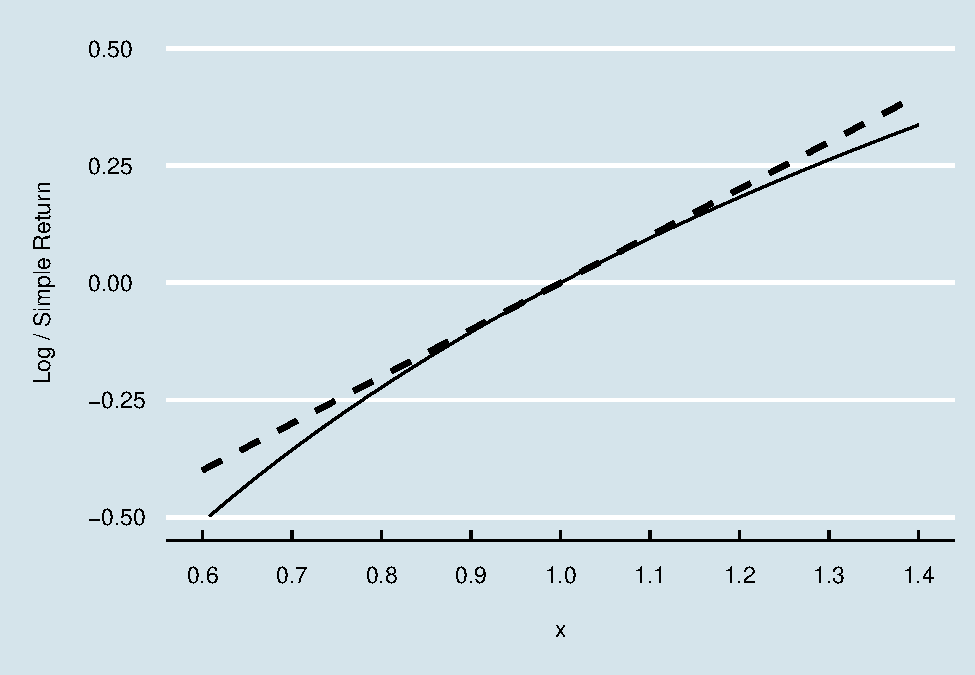
\includegraphics[width=0.8\linewidth]{StatsAssignment_files/figure-latex/plotcurve-1}

\end{document}
